\documentclass[a4paper,11pt]{article}

\usepackage[english]{babel}
\usepackage{mathrsfs, amssymb, amsmath, amsthm, enumerate}
\usepackage{verbatim,graphicx,geometry,bbm}
%\usetikzlibrary{arrows}
\usepackage[utf8]{inputenc}
\usepackage{authblk}
\usepackage[round]{natbib}
\bibliographystyle{plainnat}

\usepackage{hyperref}

\makeatletter
\def\@biblabel#1{\hspace*{-\labelsep}}
\makeatother
\geometry{left=1in,right=1
in,top=1in,bottom=1in}
\newdimen\dummy
\dummy=\oddsidemargin
\addtolength{\dummy}{72pt}
\marginparwidth=.5\dummy
\marginparsep=.1\dummy


\newcommand{\E}{\mathbb{E}}
\newcommand{\Var}{\mathrm{Var}}
\newcommand{\plim}{\overset{p}{\longrightarrow}}
\newcommand{\dlim}{\overset{d}{\longrightarrow}}

\begin{document}

\section*{50 years subsidy}

\begin{itemize}
\item Figure 1 summarizes results; it compares the welfare gains of having subsidies for new technologies and new combinations.
\item Because Figure 1's scale does not show it properly, Figure 2 plots only the new technologies subsidy welfare compared to the baseline welfare. Here we can see that the welfare is increasing in the subsidy.
\item Figure 3 repeats Figure 2, but for new combinations. It highlights the non-monotonic shape of welfare gains as a function of the subsidy.
\end{itemize}

\paragraph{Comments}
The new combination subsidy basically takes over after a subsidy of about 50\%. My guess is that everyone that would do refinements now switches to new combinations. This increases the welfare gains, but might hurt the growth of consumption if inventors who were doing new technologies revert to new combinations. If this is the case, then the welfare gains might be different if we consider more periods into the future.

\begin{figure}[h!]
\centering
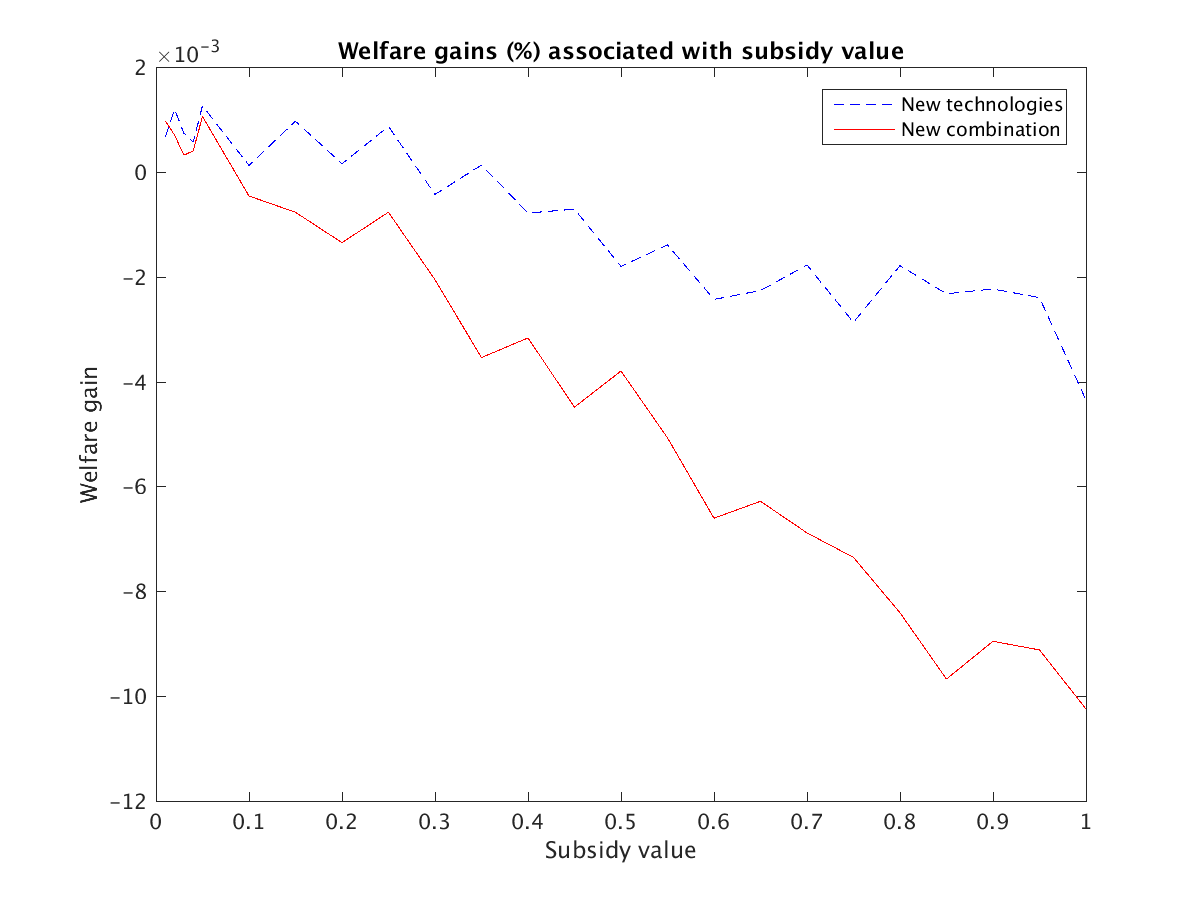
\includegraphics[scale=.6]{code/welfare_pp}
\caption{Welfare gains in percentage points.}
\end{figure}

\begin{figure}[h!]
\centering
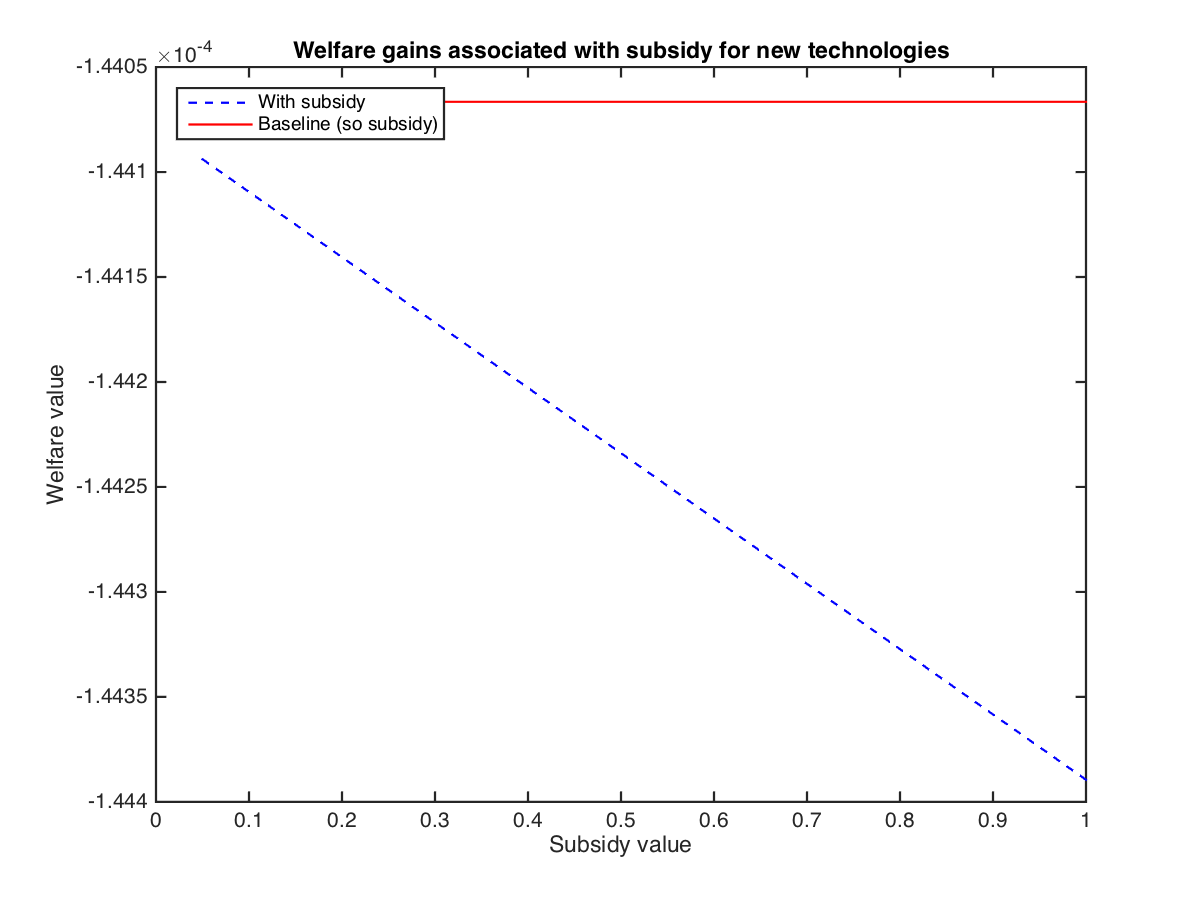
\includegraphics[scale=.6]{code/welfare_NT}
\caption{Welfare with new technologies subsidy compared to baseline in absolute values}
\end{figure}

\begin{figure}[h!]
\centering
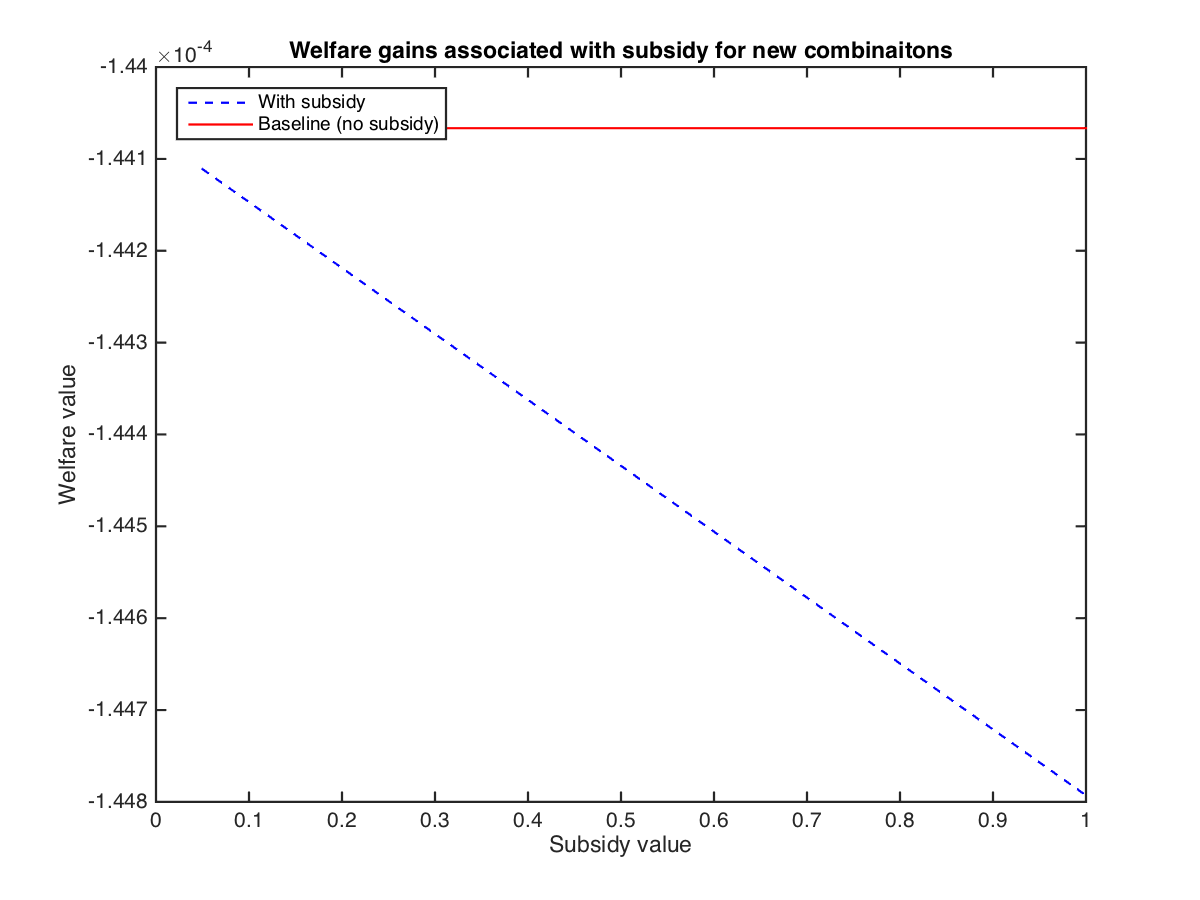
\includegraphics[scale=.6]{code/welfare_NC}
\caption{Welfare with new combinations subsidy compared to baseline in absolute values}
\end{figure}


\end{document}